\chapter{Methodology}%
\label{chap:Methodology}


In this chapter, we introduce an approach to dynamic windowing 
in data stream processing 
with the following improvements to fixed size windows; 
\begin{enumerate*}[label=(\alph*)]
    \item stream-characteristic-aware processing 
    \item adaptive window sizes, and 
    \item high throughput with low latency processing. 
\end{enumerate*}

Existing fixed size windows are inflexible when the characteristics of a data stream,  
such as the stream rate, change over time. Either the window size is 
too small to produce any output or too large which leads to high memory usage when 
the stream rate is high. Furthermore, fixed size windows only process the 
records inside the window at fixed interval (usually equal to the size of the window). 
This leads to high latency proportional to the window size. As a consequence, 
it causes unnecessarily high latency in some operations, where records could be processed once they arrive inside 
the window. One example of such operation is the join operator, where the joined 
result can be emitted the moment a new record arrives inside the window. 
Solving these disadvantages leads us to our approach 
of a dynamic window, which can adjust its size during runtime,
resulting in a low latency and high throughput solution. 


This chapter will be outlined as follows. 
First, we analyse the possible sites across the different stages of 
RMLStreamer to implement our dynamic window. Next, we define which operator
(join, aggregation, etc \dots) to implement as the reference processing operator inside 
our dynamic window. Subsequently, we elaborate our dynamic window algorithm to allow 
dynamic adjustment of window sizes depending on the stream rate of the incoming records.  
Finally, we give a brief overview of our reference implementation.



\section{Analysis for the implementation site}
\label{sec:analysis implementation site}
There are two possible sites to implement our dynamic window; 
\emph{before} or \emph{after} the mapping of non-RDF to RDF data. There are different trade-offs for choosing one 
over the other. 

\paragraph{After the mapping process}%
Implementing the windowing operations after the mapping process allows the 
possibility of applying graph processing operators in the window; the input data for 
the windows will be RDF triples from the mapping process. 

However, it comes with a major disadvantage. All the attributes required in the operator 
will have to be mapped in the mapping stage to their corresponding triple statements. 
This could lead to an explosion in the number of triple statements being generated, increasing 
the network cost of sending the data to the windowing stage. High latency processing in 
the mapping stage will also occur if the amount of attributes required by 
the operator is sufficiently large enough. 


\paragraph{Before the mapping process}%
\label{par:Before the mapping process}
To mitigate the explosion of triple statements after the mapping process, we could implement 
the windowing right before the mapping process. A reduction in the amount of 
data needed to be processed in the mapping stage could be achieved by operators 
such as \emph{filter} or \emph{joins} in the windowing stage. Furthermore, direct 
access to the raw data allows more arbitrary transformations to be applied such as 
those specified in FnO~\cite{fno_ben}, without the loss of 
information due to mapping process. 

If graph processing operations are required, we could delegate the processing computations to 
existing state-of-the-art RDF stream processing engines by attaching them at the output of 
RMLStreamer. In conclusion, it is ideal to implement the windowing before the mapping process. 


\begin{figure}[htpb]
    \centering
    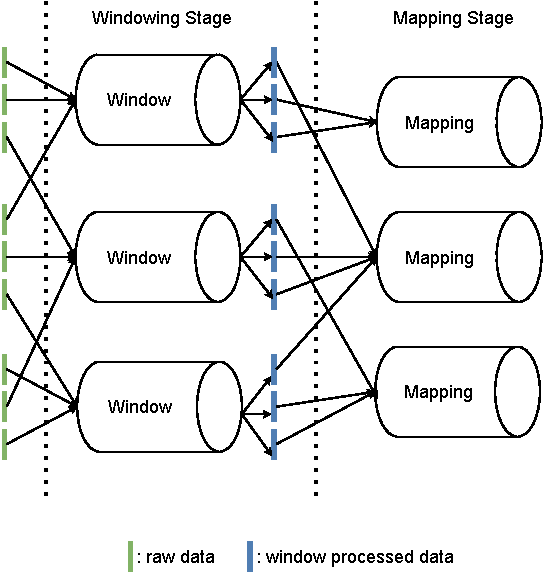
\includegraphics[width=0.7\linewidth]{fig/window_site.pdf}
    \caption{Implementation of windowing stage \textbf{before} the mapping stage. The blue blocks 
    are chunks of processed records of an \emph{operator} (join, aggregation, etc\dots) in the windows. 
    The green blocks are raw data chunks from the 
    ingestion stage (Figure~\ref{fig:rml-parallel-arch}). }%
    \label{fig:fig/s}
\end{figure}


\section{Operator inside window}
\label{sec:Operator inside window}
Which type of operation is suitable for our dynamic window? 
In the context of this work with RMLStreamer, we will have to consider optimizing the 
\emph{join} operation.

RDF mapping engines focus 
on just mapping the input to RDF compliant formats without 
applying complex stream processing queries like \emph{aggregations} and 
\emph{reductions}. These stream processing queries, if required, could be 
delegated to RDF stream processing frameworks processing RDF data streams.
Therefore, we focus on a reference implementation of dynamic windows with 
stream joins as part of the mapping process of heterogeneous data streams 
to RDF data streams.




\section{Dynamic Window}%z
\label{sec:Dynamic Window}
A dynamic window is a type of partitioned window (Chapter~\ref{sec:Partitioned Window}).
We define it as a group of subwindows, which update their sizes dynamically according to the characteristics 
of the data stream. It groups the incoming streams into different partitions first, according to 
the \emph{key} attribute value of the records. Subsequently, these grouped records are assigned 
to individual subwindows. These subwindows adjust their own size independently from each other 
at each update cycle. Furthermore, the subwindows will be independent from each other such 
that the stream rate is local to the attribute value for which each subwindow is responsible. 

We shall first extend the notations in Chapter~\ref{sec:window_notations} to aid in the 
elaboration of our dynamic window. Finally, the full algorithm for dynamic windowing 
is described in detail in pseudo code. 


\paragraph{Notations}

Similar to the notations in Chapter~\ref{sec:window_notations}, we extend the 
notations used in~\cite{generic_window_sem}. 
$W^{a} = \{ W^{a=v} | v \in \{r.a | r \text{ is a record in } W^a\}\}$ is a dynamic window, 
where $a$ represents a \emph{key} attribute. $|W^a|$ is the number of subwindows 
in $W^a$, and $W^{a=v}$ represents a subwindow associated with a \emph{key} attribute value 
$v$. Each subwindow is defined as $W^{a=v} = \{r_{i}^{a=v} | i \in [0\dots|W^{a=v}|-1]\}$, 
where $r_{i}^{a=v}$ are ordered from the newest to the oldest starting from 
$0\dots n$ with the oldest record being $r_{n}^{a=v}$ with $n = |W^{a=v}|-1$. 
The current record to be put into the subwindow $W^{a=v}$ is denoted as $r_{c}^{a=v}$. 
The \textbf{event} timestamp associated with the record $r_{i}^{a=v}$ is denoted as 
$\tau(r_{i}^{a=v})$. 

The two streams to be joined are denoted as $S_P$ and $S_C$, for 
streams representing the parent triple map and child triple map respectively~\cite{rml}. 
The number of records in the subwindow $W^{a=v}$ from $S_P$, and $S_C$ are respectively 
denoted as $|S_{P}^{a=v}|$, and $|S_{C}^{a=v}|$. The list states, 
a data structure to hold the records from $S_P^{a=v}$ and $S_C^{a=v}$, 
are respectively denoted as $List_P^{a=v}$ and $List_C^{a=v}$. 
We also denote the 
pseudo maximum size of the list states  $List_P^{a=v}$ and $List_C^{a=v}$
as $Size(List_P^{a=v})$ and $Size(List_C^{a=v})$ respectively. A record from $S_P^{a=v}$ or $S_C^{a=v}$  
is denoted as $r_i^{a=v,P}$ or $r_i^{a=v, C}$ respectively.

We also define a threshold $\epsilon$ used to check if the window size needs 
to be adjusted based on the join cost $m$. Generally, if $\epsilon = 1.5$, it represents 
the threshold where the number of records inside a subwindow, $W^{a=v}$, 
is $1.5$ times the size of $Size(List_P^{a=v}) + Size(List_C^{a=v})$.  

\subsection{Dynamic window join}
\label{sub:Dynamic window join}

The join algorithm used, is a variant of Symmetric Hash Join~\cite{symmetric_hash_join}. 
The subwindow themselves work like a hash table, containing records with a 
specific \emph{key} --- since they are \emph{partitioned} (Chapter~\ref{sec:Partitioned Window}). 
The records are joined by probing the relevant stream and generating the 
joined result. 

We will work through a simple example when a record $r_c$ arrives 
inside a subwindow $W^{a=v}$. For ease of writing, we omit $a=v$ in our notations. 


\begin{exmp}    
    Provided the incoming record is $r_c^{P}$, we first insert 
    it into $List_P$. Subsequently, we probe for 
    $\forall i, r_i^C \in List_C$, and join all $r_i^C$ found, with $r_c^P$
    as tuples of $(r_c^P, r_i^C) \text{ with } \forall i, r_i \in List_C$.
    Similar steps are executed for $r_c^C$. 
\end{exmp}





\subsection{Dynamic window sizing}%
\label{sub:Dynamic window sizing}
For each subwindow $W^{a=v}$, the following configuration parameters 
are provided: 

\begin{itemize}
    \item $\Delta n$: the \textbf{initial} interval of time before the next eviction trigger (Chapter \ref{chap:windows}). 
    \item $\epsilon_u$: the upper limit for threshold $\epsilon$.
    \item $\epsilon_l$: the lower limit for threshold $\epsilon$. 
    \item $U$: the upper limit for the window size. 
    \item $L$: the lower limit for the window size. 
\end{itemize}



For ease of writing, we will omit $a=v$ to specify the \emph{key} attribute associated 
with the subwindow. 
Therefore, the following events happen for every subwindow $W^{a=v}$ independently from 
each other. 

Since we are implementing the join operator, the trigger event is fired when  
$r_c$ arrives, and the join operation in Chapter~\ref{sub:Dynamic window join} is 
executed. 


The eviction trigger is fired every time when the current watermark (Section \ref{ssub:Watermarking}) 
$w \ge |W| + \Delta n$. At each eviction trigger we calculate the 
the cost for each \emph{list states} $List_P$ and $List_C$, containing the records from $S_P$ and $S_C$
respectively. The cost for $cost(List_P) = |S_P|/Size(List_P)$, idem for $cost(List_C)$. 
The total cost is $m = cost(List_P) + cost(List_C)$ and it is checked against thresholds $\epsilon_l$ and $\epsilon_u$. If  $\epsilon_l \le m \le \epsilon_u$, 
$\Delta n$ stays the same, otherwise it will be adjusted accordingly. This provides some stability 
in window sizing by keeping the same size, if the cost lies within the thresholds. 
The higher $m$, the higher the stream rate. Thus, the subwindow needs to be frequently 
evicted and lower $\Delta n$ to reduce memory usage. There is also a limit on the 
minimum and maximum window sizes, $L$ and $U$ respectively, to ensure that the window 
size $\Delta n$ does not keep growing or shrinking in size infinitely, in worst case scenario. 
The sizes of the list states 
are also updated according to $Size(List_P) = Size(List_P) * cost(List_P) + 0.5$.
Similarly for $Size(List_C)$. 
Hence the dynamic window maintains an 
ideal size by adjusting $\Delta n, Size(List_P)$ and $Size(List_C)$ according to 
the stream rate. The pseudo code for the eviction algorithm is presented in Algorithm~\ref{alg:dynamic_eviction}.

This algorithm for the dynamic window is an adaptation of the VC-TWindow~\cite{vctw_join} with 
improvements for stability in window sizing, clarity in the metrics used for updates, and localization 
of window size update to each subwindow.  

\begin{algorithm}[htbp]
    \DontPrintSemicolon
    \KwData{$\Delta n, \epsilon_u, \epsilon_l, U, L, List_P, List_C, S_P, S_C$}

    \tcp{Note: cost(..) is ratio for how "full" a list-state is} 
    $cost(List_P) = |S_P| / Size(List_P)$      \tcp*{Calculate the cost (ratio) of list-state P } 
    $cost(List_C) = |S_C| / Size(List_C)$      \tcp*{Calculate the cost (ratio) of list-state C } 


    total cost $ m = cost(List_P) + cost(List_C)$  
  
    \If{$m > \epsilon_u$} 
    {
        \tcp{the cost is too high, shrink the window size and adjust list-states}
        $\Delta n = \Delta n / 2 $ 
        
        $Size(List_P) = Size(List_P) * (cost(List_P) + 0.5)$  

        $Size(List_C) = Size(List_C) * (cost(List_C) + 0.5)$  
    }
    \ElseIf{$m < \epsilon_l$}
    {
        \tcp{the cost is too low, increase the window size and adjust list-states}
        $\Delta n = \Delta n * 2$ 

        $Size(List_P) = Size(List_P) * (cost(List_P) + 0.5)$  

        $Size(List_C) = Size(List_C) * (cost(List_C) + 0.5)$  
    }

    clean both $List_C \text{ and } List_P$
    \caption{Dynamic window $onEviction$ routine}
    \label{alg:dynamic_eviction}
\end{algorithm}



\section{Implementation}%
\label{sec:Implementation}

The dynamic window is implemented for RMLStreamer 
to extend its capabilities to do simple stream processing by 
joining multiple streams. RMLStreamer is implemented in Scala 
on top of the Apache Flink framework and with Flink's easy to access, low-level APIs, 
we could easily implement our custom dynamic window.  

Furthermore, new \emph{properties} and \emph{classes} are defined to extend RML with 
support for window configurations. RML's extensibility allows us to 
define new RML vocabularies without changing the existing ones. The ontology 
definitions is rudimentary at this moment and it is used only to configure our 
window type. However, it could easily be extended to also include windo specific 
parameter configurations if required. An example of this RML mapping file for 
dynamic window can 
be found in Appendix~\ref{lst:dynamic_mapping_file}. For example, one could 
adjust the window type by changing the literal value for the property 
\emph{rmls:windowType} with either \emph{rmls:Tumbling} or \emph{rmls:DynamicWindow}. 








 




